\documentclass[12pt,a4paper]{article}
\usepackage[utf8]{inputenc}
\usepackage[spanish,es-tabla]{babel}
\usepackage{geometry}
\usepackage{graphicx}
\usepackage{multirow}
\usepackage{tabularx}
\usepackage{mathptmx}
\usepackage{fancyhdr}
\usepackage{array}
\usepackage[table]{xcolor}
\usepackage{titlesec}
\usepackage{setspace}
\usepackage{microtype}
\usepackage{lastpage}
\usepackage{booktabs}
\usepackage{enumitem}
\usepackage{amsmath}
\usepackage{amsfonts}
\usepackage{amssymb}

\graphicspath{{images/}{../images/}{./}}

\geometry{
    top=4.7cm,
    bottom=2.5cm,
    left=2.5cm,
    right=2.5cm,
    headheight=3.9cm,
    headsep=0.4cm
}

\setstretch{1.15}
\setlength{\parindent}{0pt}
\setlength{\parskip}{0.45em}
\setlength{\tabcolsep}{4pt}

\titleformat{\section}
  {\normalfont\fontsize{12}{14.5}\bfseries}{\thesection.}{0.6em}{\uppercase}
\titlespacing*{\section}
  {0pt}{1.8ex plus 0.4ex minus 0.2ex}{0.6ex plus 0.2ex}

\titleformat{\subsection}
  {\normalfont\fontsize{11.5}{13.5}\bfseries}{\thesubsection.}{0.5em}{}
\titlespacing*{\subsection}
  {0pt}{1.4ex plus 0.3ex minus 0.1ex}{0.4ex plus 0.1ex}

\titleformat{\subsubsection}
  {\normalfont\fontsize{10.5}{12.5}\bfseries\itshape}{\thesubsubsection.}{0.4em}{}
\titlespacing*{\subsubsection}
  {0pt}{1.1ex plus 0.2ex minus 0.1ex}{0.3ex plus 0.1ex}

\newcolumntype{Y}{>{\centering\arraybackslash}X}
\newcolumntype{L}{>{\raggedright\arraybackslash}X}
\newcolumntype{C}{>{\centering\arraybackslash}X}

\definecolor{headerred}{RGB}{180, 0, 0}
\definecolor{darkred}{RGB}{140, 0, 0}
\definecolor{lightgraybg}{RGB}{248, 248, 248}
\definecolor{tableheader}{RGB}{232, 238, 246}

\newcommand{\docCodigo}{TI-SIGE-ENT-S1-004}
\newcommand{\docVersion}{1.0}
\newcommand{\docProceso}{PLANIFICACIÓN Y GESTIÓN DEL ALCANCE}
\newcommand{\docElaboracion}{19/08/2026}
\newcommand{\docRevision}{PENDIENTE DE REVISIÓN}
\newcommand{\docTitulo}{DEFINICIÓN FORMAL DEL ALCANCE, RESTRICCIONES, SUPUESTOS Y OBJETIVOS}
\newcommand{\docOrganizacion}{FACULTAD DE INGENIERÍA EN SISTEMAS, ELECTRÓNICA E INDUSTRIAL}
\newcommand{\docSubOrganizacion}{CARRERA DE INGENIERÍA DE SOFTWARE}

\newcommand{\encabezadofrecuente}{%
    \renewcommand{\arraystretch}{1.15}%
    \noindent\makebox[\textwidth][c]{%
    \begin{tabularx}{\textwidth}{|>{\centering\arraybackslash}m{2.8cm}|Y|>{\centering\arraybackslash}m{4.8cm}|}
        \hline
        \multirow{4}{2.8cm}{\centering\raisebox{-1.15cm}{
\includegraphics[width=2.5cm,height=2.0cm,keepaspectratio]{images/logo.png}}}
        & \textbf{\fontsize{9}{11}\selectfont \docOrganizacion} 
        & \textbf{\fontsize{8}{10}\selectfont CÓDIGO:} \fontsize{8}{10}\selectfont \docCodigo \\
        \cline{3-3}
        & \textbf{\fontsize{8.5}{10.5}\selectfont \docSubOrganizacion} 
        & \textbf{\fontsize{8}{10}\selectfont VERSIÓN:} \fontsize{8}{10}\selectfont \docVersion \\
        \cline{2-3}
        & \textbf{\fontsize{8}{10}\selectfont PROCESO:} \fontsize{8}{10}\selectfont \docProceso 
        & \textbf{\fontsize{8}{10}\selectfont ELABORACIÓN:} \fontsize{8}{10}\selectfont \docElaboracion \\
        \cline{2-3}
        & \textbf{\fontsize{8.5}{10.5}\selectfont \docTitulo} 
        & \textbf{\fontsize{8}{10}\selectfont ÚLTIMA REVISIÓN:} \fontsize{8}{10}\selectfont \textbf{\textcolor{darkred}{\docRevision}} \\
        \hline
    \end{tabularx}%
    }%
}

\pagestyle{fancy}
\fancyhf{}
\fancyhead[C]{\encabezadofrecuente}
\fancyfoot[C]{\fontsize{10}{12}\selectfont Página \thepage\ de \pageref{LastPage}}
\renewcommand{\headrulewidth}{0pt}

\begin{document}

\section{Título}
\textbf{Denominación del Entregable:} Declaración del Alcance del Proyecto, Restricciones y Matriz de Trazabilidad (EDT 1.4)

\vspace{0.15cm}
\noindent
\textbf{Ficha Técnica de Identificación:}
\begin{itemize}[leftmargin=1.5em, itemsep=1.5pt, topsep=1.5pt]
    \item \textbf{Código Documental:} \docCodigo \quad | \quad \textbf{Versión:} \docVersion
    \item \textbf{Institución:} Universidad Técnica de Ambato (UTA) -- FISEI
    \item \textbf{Carrera:} Ingeniería de Software (Séptimo Semestre "A")
    \item \textbf{Módulo Académico:} Gestión de Proyectos de Software
    \item \textbf{Docente Tutor:} Ing. Paulo Torres
    \item \textbf{Fecha de Elaboración:} \docElaboracion \quad | \quad \textbf{Estado:} \textbf{\textcolor{darkred}{En Elaboración / Pendiente de Revisión}}
    \item \textbf{Período de Ejecución:} Semana 1 (19/08/2026 al 21/08/2026)
    \item \textbf{Responsables:} Steeven Toala (Líder / Arquitecto) y Heidy Villavicencio (Analista)
\end{itemize}

\section{Introducción}
La delimitación precisa del alcance constituye un pilar esencial en la ingeniería de software para prevenir el desvío de objetivos (\textit{Scope Creep}). En este documento se formalizan los objetivos generales y específicos bajo criterios SMART, se establece la frontera operativa entre los componentes dentro y fuera del alcance (\textit{In-Scope vs. Out-of-Scope}) y se estructuran las restricciones presupuestarias, tecnológicas y temporales del proyecto \textbf{SIGE} para la FISEI UTA.

\section{Objetivos del Proyecto}

\subsection{Objetivo General}
Planificar, diseñar e implementar el sistema web institucional \textbf{SIGE}, automatizando la elaboración, seguimiento de matrices de actividades, revisión con observaciones granulares y aprobación multinivel de los planes de trabajo e informes institucionales basados en el Sistema de Gestión de Calidad (SGC), integrando una capa de asistencia mediante Inteligencia Artificial gratuita y local.

\subsection{Objetivos Específicos}
\begin{enumerate}[leftmargin=1.5em, itemsep=2pt, topsep=2pt]
    \item \textbf{OE-01:} Formalizar los requerimientos funcionales del flujo institucional de gestión de calidad, estandarizando digitalmente los formatos oficiales vigentes de planes e informes (\texttt{UTA-SGC-A-2-1-P7-T1} y \texttt{UTA-SGC-A-2-1-P7-T2}).
    \item \textbf{OE-02:} Diseñar una interfaz responsiva, sobria y moderna estructurada en pestañas con editor de texto enriquecido (TipTap) y paleta de colores institucional Azul y Blanco.
    \item \textbf{OE-03:} Implementar en backend reglas de validación deterministas (\textit{Validation Gates}) para el control estricto de matrices, porcentajes y evidencias obligatorias.
    \item \textbf{OE-04:} Construir el módulo de comité de revisión con observaciones por párrafo, dictámenes oficiales y flujo de firmas secuenciales parametrizable en cascada.
    \item \textbf{OE-05:} Integrar una arquitectura de Inteligencia Artificial híbrida (LanguageTool en Docker local para corrección sintáctica y Google Gemini API para asistencia semántica institucional), desacoplada y sin costos de suscripción comercial.
    \item \textbf{OE-06:} Desarrollar el motor de exportación a formatos oficiales Word/PDF y el registro inmutable de auditoría con firmado criptográfico SHA-256.
\end{enumerate}

\section{Declaración del Alcance (In-Scope vs. Out-of-Scope)}

\subsection{Dentro del Alcance (In-Scope)}
\begin{itemize}[leftmargin=1.5em, itemsep=2pt]
    \item \textbf{Formatos Oficiales SGC:} Digitalización determinista del Plan de Trabajo (\texttt{UTA-SGC-A-2-1-P7-T1}) y del Informe de Cumplimiento (\texttt{UTA-SGC-A-2-1-P7-T2}).
    \item \textbf{Editor Wizard Modular:} Interfaz de redacción estructurada en 6--7 pestañas ordenadas lógicamente con autoguardado asíncrono.
    \item \textbf{Validation Gates:} Bloqueo de avance en caso de matrices incompletas, fechas inconsistentes o desvíos sin justificar.
    \item \textbf{Almacenamiento de Evidencias MinIO S3:} Carga y enlace seguro de archivos probatorios mediante URLs prefirmadas.
    \item \textbf{Circuito Secuencial de Firmas Digitales:} Flujo jerárquico en cascada oficial (Docente Elaborador $\rightarrow$ Coordinador de Área $\rightarrow$ Coordinador de Carrera).
    \item \textbf{Asistente Ortográfico Local:} Contenedor Docker local con LanguageTool para corrección ortográfica y gramatical sin costos de red.
    \item \textbf{Asistencia Semántica Institucional:} Conectividad con Google Gemini API (Free Tier institucional) para síntesis de textos y sugerencias contextuales.
    \item \textbf{Generación Oficial de Documentos:} Motor QuestPDF y OpenXML para exportación fidedigna a PDF y Word \texttt{.docx}.
    \item \textbf{Historial y Auditoría SHA-256:} Versionado autoincremental (\texttt{V01}, \texttt{V02}) y registro inmutable de transacciones.
\end{itemize}

\subsection{Fuera del Alcance (Out-of-Scope)}
\begin{itemize}[leftmargin=1.5em, itemsep=2pt]
    \item Módulo de nómina, cálculo de salarios o pago financiero de horas docentes.
    \item Control biométrico de asistencia física a aulas o laboratorios.
    \item Gestión de matrículas, actas de notas y calificaciones de estudiantes (mantenido por el SGA central).
    \item Suscripciones comerciales de pago por usuario o modelos LLM comerciales de alto costo (OpenAI, Claude).
\end{itemize}

\begin{figure}[htbp]
    \centering
    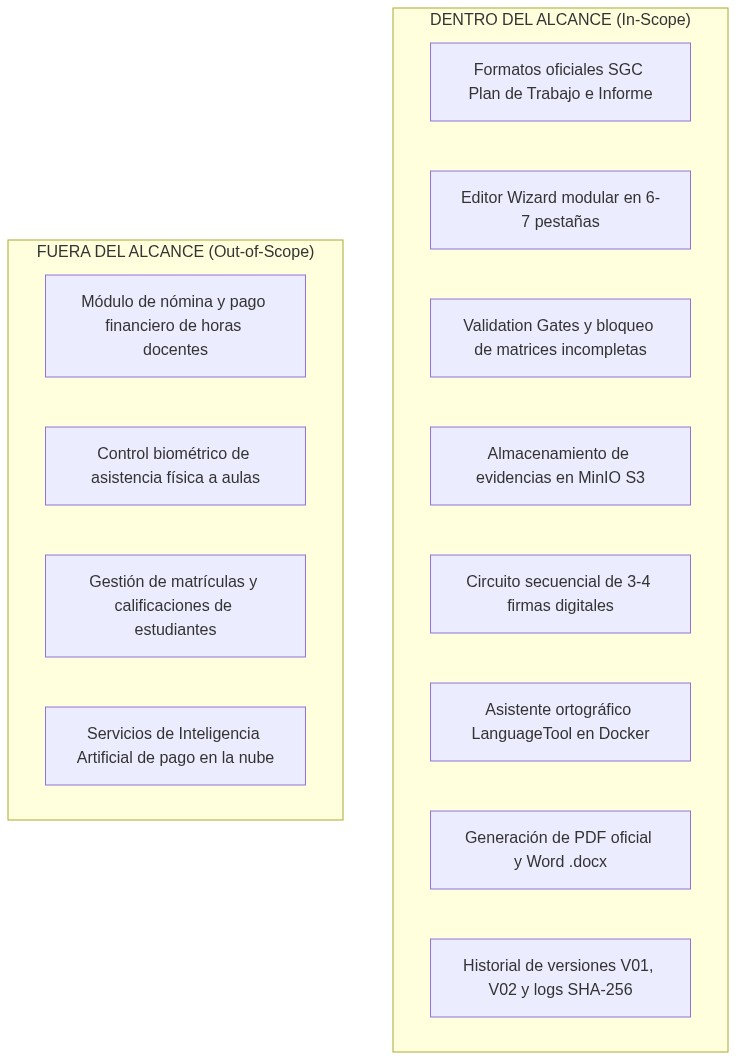
\includegraphics[width=0.75\textwidth,height=6.5cm,keepaspectratio]{images/s1_04_alcance.png}
    \caption{Fronteras Operativas del Sistema SIGE (In-Scope vs. Out-of-Scope).}
    \label{fig:s1_04_scope}
\end{figure}

\section{Restricciones y Supuestos del Proyecto}

\subsection{Restricciones del Proyecto}
\begin{enumerate}[leftmargin=1.5em, itemsep=2.5pt]
    \item \textbf{Restricción Presupuestaria:} El presupuesto de inversión directa está limitado a \textbf{\$630.30 USD} para infraestructura cloud (VPS, PostgreSQL gestionado, MinIO, dominio/SSL, SMTP y licencias de desarrollo). La mano de obra se valoriza en \textbf{\$0.00 USD} como aporte académico de los 4 estudiantes de ingeniería.
    \item \textbf{Restricción Temporal:} El cronograma contempla una duración fija de \textbf{80 días calendario (12/08/2026 -- 30/10/2026)} distribuido en 5 fases de ejecución ágil según la estructura de desglose del trabajo (EDT).
    \item \textbf{Restricción Tecnológica:} El stack opera bajo un modelo de optimización de recursos: corrección sintáctica en contenedor Docker local (LanguageTool) y asistencia semántica mediante Google Gemini API sin suscripciones comerciales de pago.
    \item \textbf{Restricción Normativa:} Los documentos generados por el sistema deben mantener correspondencia estricta con las directrices de la Dirección de Aseguramiento de la Calidad de la UTA.
\end{enumerate}

\subsection{Supuestos del Proyecto}
\begin{itemize}[leftmargin=1.5em, itemsep=2pt]
    \item Los docentes y autoridades cuentan con certificados de firma electrónica vigentes emitidos por entidades certificadoras acreditadas en el país (FirmaEC, Security Data, Banco Central, etc.).
    \item El servidor VPS provisto cuenta con capacidades mínimas de 4 vCPUs y 8 GB RAM para soportar los contenedores de PostgreSQL, MinIO y LanguageTool.
    \item Las autoridades de la facultad facilitarán oportunamente las sesiones de validación y pruebas de aceptación de usuario.
\end{itemize}

\section{Matriz de Trazabilidad de Requerimientos (RTM)}
A continuación se detalla la vinculación formal entre los objetivos específicos del proyecto y los requerimientos funcionales aprobados:

\begin{table}[htbp]
\centering
\small
\begin{tabularx}{\textwidth}{|>{\hsize=0.35\hsize\bfseries\centering\arraybackslash}X|>{\hsize=0.85\hsize}X|>{\hsize=0.9\hsize}X|>{\hsize=0.9\hsize}X|}
    \hline
    \rowcolor{tableheader}
    Obj. Específico & Requisitos Funcionales Asociados & Entregable de Verificación & Criterio de Aceptación \\
    \hline
    \textbf{OE-01} & RF-01, RF-02, RF-04, RF-05, RF-06 & SRS IEEE 830 y Matriz de Casos de Uso & Aprobación formal del documento por el docente de la cátedra. \\
    \hline
    \textbf{OE-02} & RF-07, RF-08, RF-09, RF-16 & Prototipos Figma y Componentes React 19 & Interfaz con navegación por pestañas funcional, sobria y accesible. \\
    \hline
    \textbf{OE-03} & RF-10, RF-11, RF-12, RF-13, RF-14 & Middleware FluentValidation en .NET 9 & Bloqueo determinista de guardado si faltan evidencias o ponderaciones. \\
    \hline
    \textbf{OE-04} & RF-17, RF-18, RF-19, RF-20, RF-21 & Módulo de Comité y Circuito de Firmas & Flujo secuencial verificado sin omisión de firmas intermedias en cascada. \\
    \hline
    \textbf{OE-05} & RF-15 & Contenedor LanguageTool en Docker & Corrección ortográfica local funcional sin peticiones externas de pago. \\
    \hline
    \textbf{OE-06} & RF-22, RF-23, RF-24 & Módulo QuestPDF, OpenXML y Logs SHA-256 & Documentos exportados idénticos a los formatos oficiales del SGC. \\
    \hline
\end{tabularx}
\caption{Matriz de Trazabilidad de Requerimientos (RTM) del Sistema SIGE.}
\label{tab:s1_04_rtm}
\end{table}

\vspace{0.3cm}

% =============================================================
% FIRMAS DE RESPONSABILIDAD
% =============================================================
\section{Firmas de Responsabilidad}

\noindent
\renewcommand{\arraystretch}{1.2}
\begin{tabularx}{\textwidth}{|>{\raggedright\arraybackslash}m{2.9cm}|>{\raggedright\arraybackslash}X|>{\centering\arraybackslash}m{4.6cm}|>{\centering\arraybackslash}m{2.3cm}|}
    \hline
    \rowcolor{headerred}
    \textcolor{white}{\textbf{ACCIÓN}} & \textcolor{white}{\textbf{NOMBRE Y CARGO}} & \textcolor{white}{\textbf{FIRMA}} & \textcolor{white}{\textbf{FECHA}} \\
    \hline
    \textbf{Elaborado por:} & Steeven Toala\newline \textit{Líder de Proyecto / Arquitecto Software} & \parbox[c]{4.4cm}{\centering\vspace{4pt}
\includegraphics[height=1.5cm,width=4.0cm,keepaspectratio]{images/firma_steveen.png}\vspace{4pt}} & 19/08/2026 \\
    \hline
    \textbf{Revisado por:} & Steeven Toala\newline \textit{Líder de Proyecto / Arquitecto Software} & \parbox[c]{4.4cm}{\centering\vspace{10pt}\textbf{\textcolor{gray!80}{\scriptsize [ PENDIENTE DE REVISIÓN ]}}\vspace{10pt}} & \textbf{\textcolor{gray!90}{Pendiente}} \\
    \hline
    \textbf{Aprobado por:} & Ing. Paulo Torres\newline \textit{Docente Tutor - Gestión Proyectos Software} & \parbox[c]{4.4cm}{\centering\vspace{10pt}\textbf{\textcolor{gray!80}{\scriptsize [ PENDIENTE DE APROBACIÓN ]}}\vspace{10pt}} & \textbf{\textcolor{gray!90}{Pendiente}} \\
    \hline
\end{tabularx}

\vspace{0.4cm}

% =============================================================
% CONTROL DE CAMBIOS
% =============================================================
\section{Control de Cambios}

\noindent
\renewcommand{\arraystretch}{1.2}
\begin{tabularx}{\textwidth}{|>{\hsize=0.45\hsize\centering\arraybackslash}X|>{\hsize=1.55\hsize\raggedright\arraybackslash}X|>{\hsize=1.2\hsize\raggedright\arraybackslash}X|>{\hsize=0.8\hsize\centering\arraybackslash}X|}
    \hline
    \rowcolor{gray!20}
    \textbf{Versión} & \textbf{Descripción del cambio} & \textbf{Responsable del cambio} & \textbf{Fecha de aprobación} \\
    \hline
    1.0 & Definición formal del alcance, restricciones, supuestos y matriz RTM / Pendiente de revisión & Steeven Toala & \textbf{\textcolor{gray!90}{Pendiente de Revisión}} \\
    \hline
\end{tabularx}

\vspace{0.4cm}

\section{Anexos}
\subsection*{Anexo 1: Registro de Restricciones de Infraestructura y Servidor}
Especificaciones técnicas de hardware del servidor VPS: 4 vCPUs, 8 GB RAM, 160 GB NVMe y configuración de firewall perimetral para PostgreSQL, MinIO y LanguageTool.

\end{document}
